% ============================================================
% 7. Design
% ============================================================
\chapter{Design}\label{ch:design}

\section{BCE Architecture (VOPC)}

CiboAmico follows the \textbf{Boundary--Control--Entity} pattern. The VOPC
(view of participating classes) respects the following rules:
\begin{itemize}
    \item each use case owns exactly \textbf{one application controller};
    \item boundaries exchange data with controllers \textbf{exclusively via
    beans (DTO)}: no entity reaches the view;
    \item controllers are \textbf{stateless}: the current user is passed as a
    parameter by the view, which resolves it from the session singleton
    (SessionManager);
    \item business logic resides in the entities.
\end{itemize}

The final model is summarised in Table~\ref{tab:vopc}. The boundary
column reports the real JavaFX/CLI view classes (two views per UC for the
double interface requirement); the bean column lists the DTOs
interposed between boundary and control (bean-only rule); the adapters are
the technical boundaries that mediate the interaction with the external
systems. The Payment Service is declared as an external actor of UC-04 for
completeness but is simulated in code (out of the evaluation scope, see
Implementation Remarks in Chapter~\ref{ch:intro}); the email notification
(UC-04/UC-06) is mediated by the \texttt{JakartaMailAdapter}.

\begin{table}[H]
\centering
\caption{BCE classes (1 controller per use case; 2 boundaries per UC for CLI+GUI double interface).}
\label{tab:vopc}
\begin{tabular}{@{}lllll@{}}
\toprule
\textbf{UC} & \textbf{Boundary (GUI/CLI)} & \textbf{Bean} & \textbf{Control} & \textbf{Main Entities} \\
\midrule
UC-01 & InventarioView / InventarioCLIView & ProdottoBean & GestisciInventarioController & ProdottoInventario \\
UC-02 & RicetteView / RicetteCLIView & RicettaBean & TrovaRicetteController & Ricetta, ProdottoInventario \\
UC-03 & ListaSpesaView / ListaSpesaCLIView & RicettaBean & GestisciListaSpesaController & Ricetta, Ingrediente \\
UC-04 & MarketplaceView / MarketplaceCLIView & OrdineBean & OrdinaProdottoController & Ordine, Prodotto \\
UC-05 & CatalogoVenditoreView / CatalogoVenditoreCLIView & ProdottoBean & GestisciCatalogoVenditoreController & Prodotto, RuoloVenditore \\
UC-06 & OrdiniRicevutiView / OrdiniRicevutiCLIView & OrdineBean & GestisciOrdiniRicevutiController & Ordine \\
UC-07 & RicetteNutrizionistaView / RicetteNutrizionistaCLIView & RicettaBean & GestisciRicetteNutrizionistaController & Ricetta, RuoloNutrizionista \\
UC-08 & AdminView / AdminCLIView & RicettaBean, UtenteBean & ApprovazioneController & RuoloVenditore, Ricetta \\
UC-11 & LoginView / LoginCLIView & AutenticazioneBean & AutenticazioneController & Utente \\
\bottomrule
\end{tabular}
\end{table}

\section{Design-Level Class Diagram}

The design-level class diagram refines the VOPC with the real Java classes,
their attributes with effective types, method signatures and the persistence
interfaces. For readability it shows the core of UC-04 and the key
architectural patterns; the remaining controllers follow the same shape.

\begin{figure}[H]
\centering
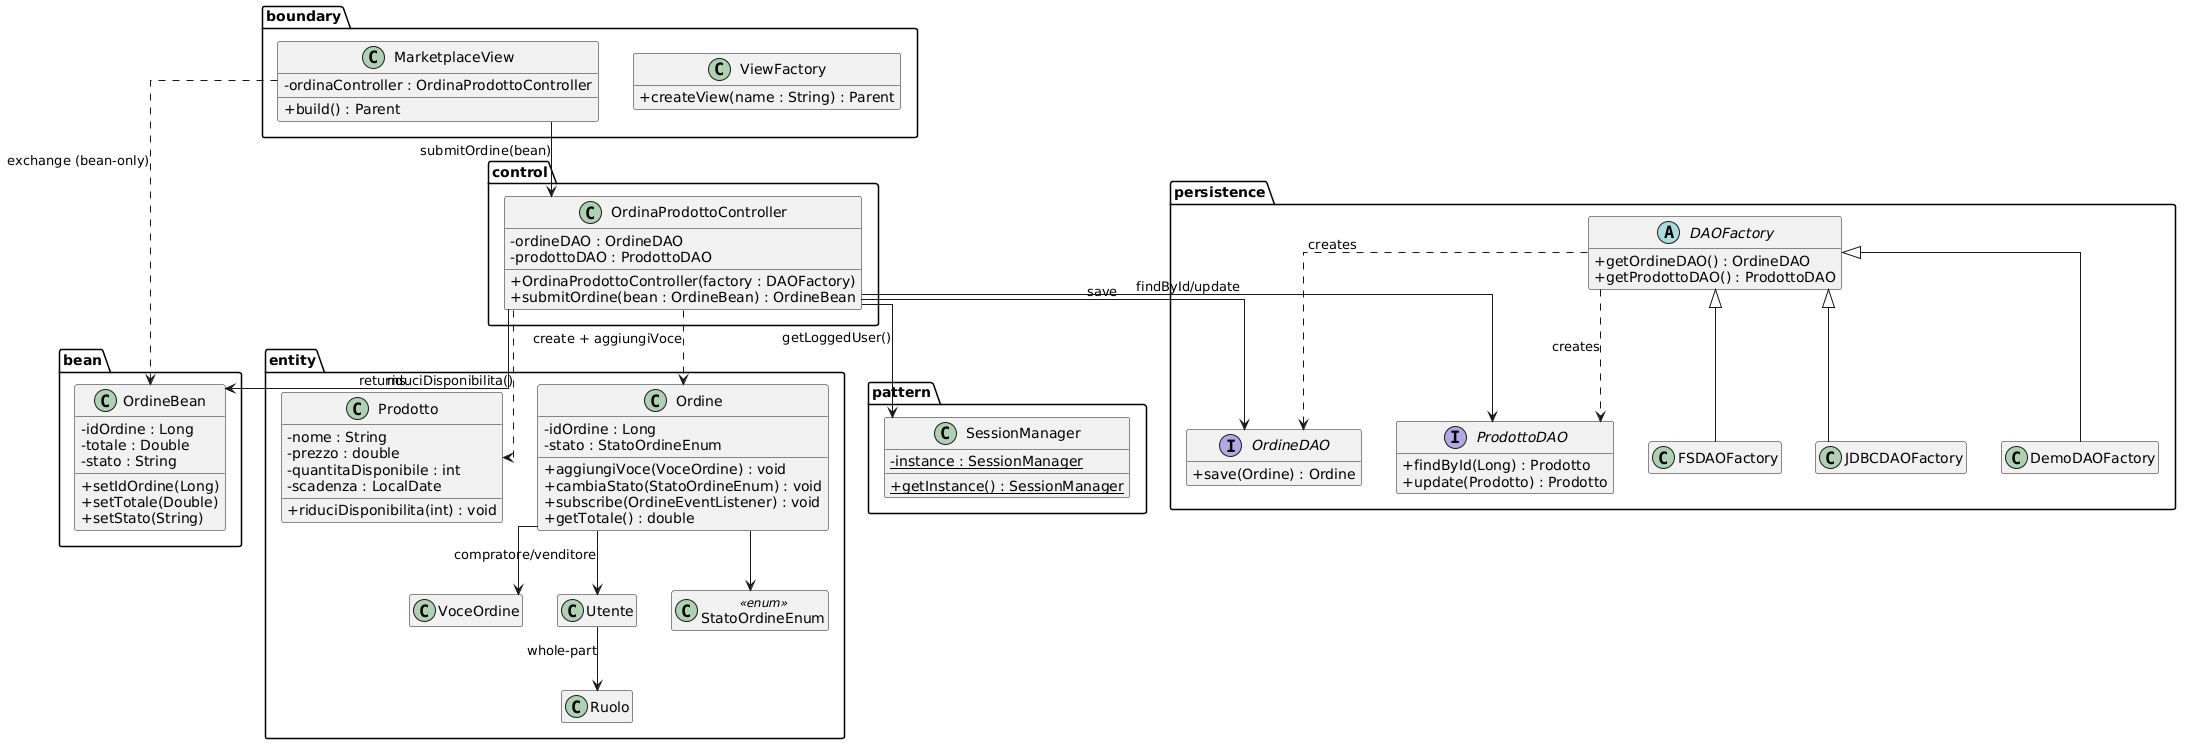
\includegraphics[width=0.98\textwidth]{figures/class-diagram-core.jpg}
\caption{Design-level class diagram: UC-04 core (boundary/bean/control/entity)
and persistence layer (DAOFactory with Demo/FS/JDBC concrete factories).}
\label{fig:classdiagram}
\end{figure}

\section{GoF Patterns}

\begin{itemize}
    \item \textbf{Singleton} -- \texttt{SessionManager},
    \texttt{ApplicationModeManager}: single session and application mode;
    \item \textbf{Lazy Initialization + caching} -- \texttt{OrdineLazyFactory}
    (Singleton with holder idiom): creates orders assigning the id from the
    DAO (Information Expert) and keeps an in-RAM cache of the session orders
    (pattern valued by De Angelis in the reference 30/30 projects);
    \item \textbf{Abstract Factory (DAO)} -- \texttt{DAOFactory} with
    \texttt{DemoDAOFactory}, \texttt{FSDAOFactory}, \texttt{JDBCDAOFactory}:
    coherent family of DAOs switchable at startup (NFR-01);
    \item \textbf{Abstract Factory (View)} -- \texttt{ViewFactory} (classe
    astratta con \texttt{getFactory()} statico, integra Singleton): sceglie a
    runtime la famiglia di boundary \texttt{JavaFXViewFactory} (GUI) oppure
    \texttt{CLIViewFactory} (CLI); i prodotti astratti sono le interfacce
    \texttt{IView} (\texttt{display()}). I controller applicativi restano
    invariati (doppia interfaccia, criterio d'esame);
    \item \textbf{Strategy} -- \texttt{StrictMatchingStrategy},
    \texttt{SubstitutionMatchingStrategy}: interchangeable matching algorithms;
    \item \textbf{Facade} -- \texttt{RicettaMatchingFacade}: single entry
    point to the recipe engine;
    \item \textbf{Observer} -- \texttt{OrdineSubject},
    \texttt{UtenteNotifier}, \texttt{VenditoreNotifier}: order-state
    notifications;
    \item \textbf{Adapter} -- \texttt{OpenFoodFactsAdapter},
    \texttt{JakartaMailAdapter}: isolates external systems;
    \item \textbf{Whole-Part} -- \texttt{Utente} aggregates \texttt{Ruolo}
    (dynamic role metamorfosi, D-02).
\end{itemize}

\subsection{Doppia interfaccia CLI/GUI}
Il sistema espone due famiglie di boundary (requisito del corso): la GUI
JavaFX e una CLI testuale. Entrambe implementano \texttt{IView.display()}
(scambio esclusivo di Bean con i controller). All'avvio
\texttt{ViewFactory.configure(\"gui\"|\"cli\")} seleziona la family e
\texttt{ViewFactory.getFactory()} (Singleton) restituisce la factory concreta:
\begin{itemize}
    \item \texttt{JavaFXViewFactory} -- delega al \texttt{Navigator}
    (\texttt{switchTo}) le schermate già registrate;
    \item \texttt{CLIViewFactory} -- viste testuali (\texttt{Scanner}) con
    menu ruolo-aware: login (UC-11), inventario (UC-01), ricette (UC-02),
    lista spesa (UC-05), marketplace (UC-06), catalogo venditore (UC-07),
    crea ricetta (UC-08), admin (UC-09/UC-12), ordini (UC-10).
\end{itemize}
Entry point: \texttt{Main [gui|cli]} (default gui).

\begin{figure}[h]
\centering
\begin{tikzpicture}[node distance=1.6cm]
\tikzstyle{absf}=[rectangle,draw,double,minimum width=3.2cm,minimum height=0.8cm]
\tikzstyle{conf}=[rectangle,draw,minimum width=3.2cm,minimum height=0.8cm]
\tikzstyle{prod}=[rectangle,draw,dashed,minimum width=3.2cm,minimum height=0.8cm]
\node (vf) [absf] {\texttt{ViewFactory} (abstract)};
\node (fx) [conf, below left=of vf] {\texttt{JavaFXViewFactory}};
\node (cli) [conf, below right=of vf] {\texttt{CLIViewFactory}};
\node (view) [prod, below=of fx, xshift=1.6cm, align=center] {\texttt{<<interface>> IView}\\ \texttt{+ display()}};
\draw[->] (vf) -- (fx);
\draw[->] (vf) -- (cli);
\draw[->, dashed] (fx) -- node[right,font=\scriptsize]{create} (view);
\draw[->, dashed] (cli) -- node[right,font=\scriptsize]{create} (view);
\node[right=2.8cm of vf, font=\scriptsize, align=left] {\texttt{+ getFactory() : ViewFactory}\\ \texttt{+ configure(String family)}};
\end{tikzpicture}
\caption{Abstract Factory delle view: doppia interfaccia CLI/GUI.}
\label{fig:view-factory}
\end{figure}

\section{Activity Diagram (UC-04)}

\begin{figure}[H]
\centering
\begin{tikzpicture}[node distance=1.2cm]
\tikzstyle{act}=[rectangle,draw,minimum width=2.2cm,minimum height=0.7cm]
\node[act] (s1) {Select product};
\node[act,right of=s1,xshift=2.6cm] (s2) {Verify availability};
\node[diamond,draw,right of=s2,xshift=2.4cm,aspect=2] (d1) {quantity available?};
\node[act,below of=d1] (s3) {Provide insufficient quantity error};
\node[act,below of=s2,yshift=-2.4cm] (s4) {Provide order summary};
\node[act,right of=d1,xshift=2.2cm] (s5) {Confirm order};
\node[diamond,draw,right of=s5,xshift=2.2cm,aspect=2] (d2) {confirmed?};
\node[act,below of=d2] (s6) {Abort};
\node[act,right of=d2,xshift=2.4cm] (s7) {Record order (CREATED)};
\node[act,right of=s7,xshift=2.2cm] (s8) {Notify vendor (async)};
\node[act,below of=s8] (s9) {End};
\draw[->] (s1)--(s2); \draw[->] (s2)--(d1);
\draw[->] (d1)--node[left]{no}(s3); \draw[->] (s3)--(s1);
\draw[->] (d1)--node[above]{yes}(s4); \draw[->] (s4)--(s5);
\draw[->] (s5)--(d2); \draw[->] (d2)--node[left]{no}(s6);
\draw[->] (d2)--node[above]{yes}(s7); \draw[->] (s7)--(s8); \draw[->] (s8)--(s9);
\end{tikzpicture}
\caption{Activity diagram of UC-04 (simplified). Other UCs follow the same
pattern: action nodes (rounded rectangles), decisions (diamonds, OR-exclusive),
no fork/join in this UC.}
\label{fig:activity}
\end{figure}

\section{Sequence Diagram (UC-04)}

\begin{figure}[H]
\centering
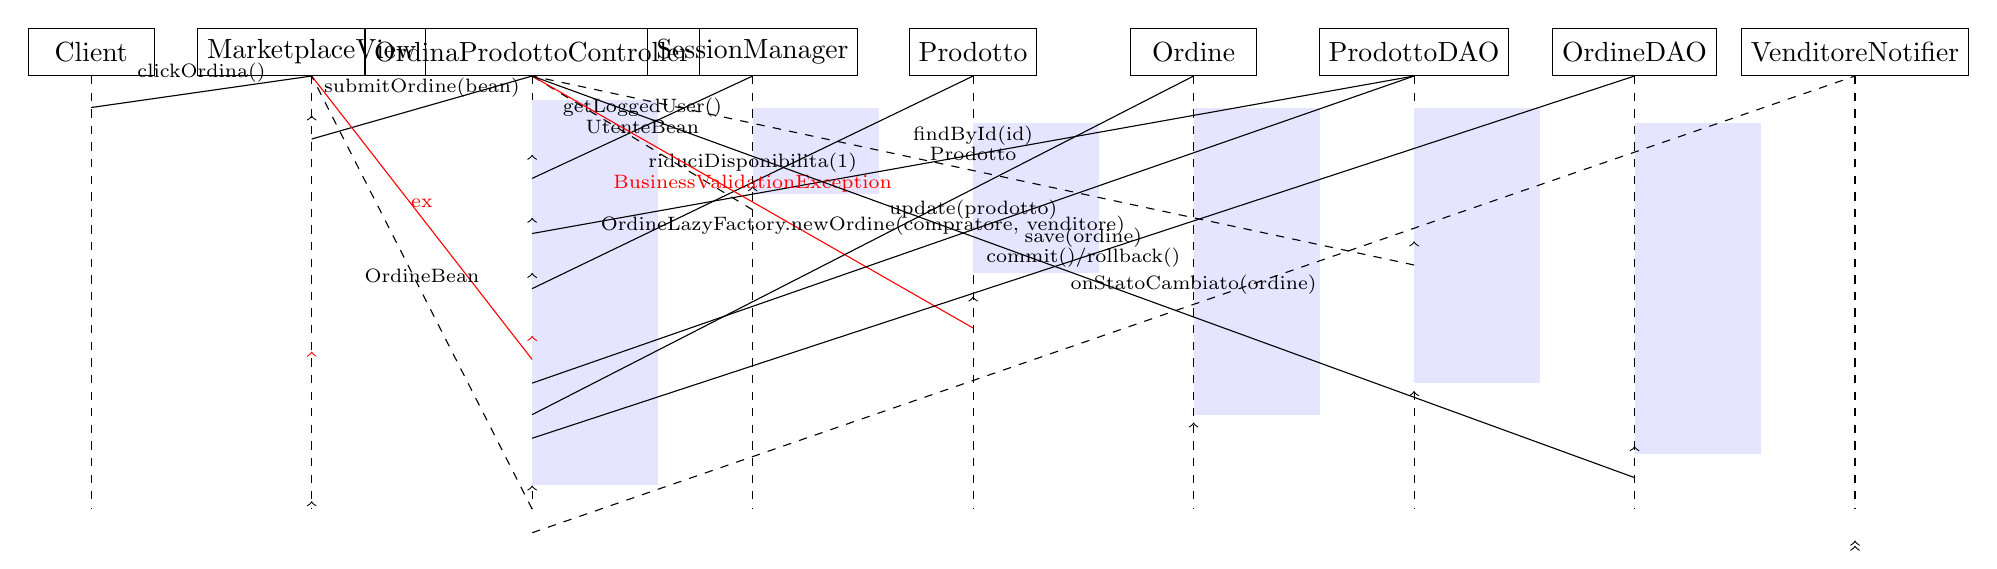
\begin{tikzpicture}
\tikzstyle{inst}=[rectangle,draw,minimum width=1.6cm,minimum height=0.6cm]
\node[inst] (c) {Client};
\node[inst,right of=c,xshift=1.8cm] (b) {MarketplaceView};
\node[inst,right of=b,xshift=1.8cm] (ctl) {OrdinaProdottoController};
\node[inst,right of=ctl,xshift=1.8cm] (sm) {SessionManager};
\node[inst,right of=sm,xshift=1.8cm] (pr) {Prodotto};
\node[inst,right of=pr,xshift=1.8cm] (e) {Ordine};
\node[inst,right of=e,xshift=1.8cm] (pdao) {ProdottoDAO};
\node[inst,right of=pdao,xshift=1.8cm] (odao) {OrdineDAO};
\node[inst,right of=odao,xshift=1.8cm] (not) {VenditoreNotifier};
% Lifelines (dashed)
\draw[dashed] (c.south) -- +(0,-5.5);
\draw[dashed] (b.south) -- +(0,-5.5);
\draw[dashed] (ctl.south) -- +(0,-5.5);
\draw[dashed] (sm.south) -- +(0,-5.5);
\draw[dashed] (pr.south) -- +(0,-5.5);
\draw[dashed] (e.south) -- +(0,-5.5);
\draw[dashed] (pdao.south) -- +(0,-5.5);
\draw[dashed] (odao.south) -- +(0,-5.5);
\draw[dashed] (not.south) -- +(0,-5.5);
% Activation boxes (rectangles on lifelines)
\fill[blue!10] (ctl.south)+(0,-1.2) rectangle +(1.6,-1.8);
\fill[blue!10] (sm.south)+(0,-1.5) rectangle +(1.6,-0.4);
\fill[blue!10] (pr.south)+(0,-2.5) rectangle +(1.6,-0.6);
\fill[blue!10] (ctl.south)+(0,-3.2) rectangle +(1.6,-1.2);
\fill[blue!10] (pdao.south)+(0,-3.9) rectangle +(1.6,-0.4);
\fill[blue!10] (e.south)+(0,-4.3) rectangle +(1.6,-0.4);
\fill[blue!10] (odao.south)+(0,-4.8) rectangle +(1.6,-0.6);
\fill[blue!10] (ctl.south)+(0,-5.2) rectangle +(1.6,-0.3);
% sync messages (full arrows)
\draw[->] (c.south)+(0,-0.4) -- (b.south)+(0,-0.5) node[midway,above]{\scriptsize clickOrdina()};
\draw[->] (b.south)+(0,-0.8) -- (ctl.south)+(0,-1.0) node[midway,above]{\scriptsize submitOrdine(bean)};
\draw[->] (ctl.south)+(0,-1.3) -- (sm.south)+(0,-1.4) node[midway,above]{\scriptsize getLoggedUser()};
\draw[->,dashed] (sm.south)+(0,-1.7) -- (ctl.south)+(0,-1.8) node[midway,above]{\scriptsize UtenteBean};
\draw[->] (ctl.south)+(0,-2.0) -- (pdao.south)+(0,-2.1) node[midway,above]{\scriptsize findById(id)};
\draw[->,dashed] (pdao.south)+(0,-2.4) -- (ctl.south)+(0,-2.5) node[midway,above]{\scriptsize Prodotto};
\draw[->] (ctl.south)+(0,-2.7) -- (pr.south)+(0,-2.8) node[midway,above]{\scriptsize riduciDisponibilita(1)};
% exception: BusinessValidationException risale alla boundary
\draw[->,red] (pr.south)+(0,-3.2) -- (ctl.south)+(0,-3.3) node[midway,above]{\scriptsize \textcolor{red}{BusinessValidationException}};
\draw[->,red] (ctl.south)+(0,-3.6) -- (b.south)+(0,-3.5) node[midway,above]{\scriptsize \textcolor{red}{ex}};
% transaction: setAutoCommit(false) + update + save + commit/rollback
\draw[->] (ctl.south)+(0,-3.9) -- (pdao.south)+(0,-4.0) node[midway,above]{\scriptsize update(prodotto)};
\draw[->] (ctl.south)+(0,-4.3) -- (e.south)+(0,-4.4) node[midway,above]{\scriptsize OrdineLazyFactory.newOrdine(compratore, venditore)};
\draw[->] (ctl.south)+(0,-4.6) -- (odao.south)+(0,-4.7) node[midway,above]{\scriptsize save(ordine)};
\draw[->] (odao.south)+(0,-5.1) -- (ctl.south)+(0,-5.2) node[midway,above]{\scriptsize commit()/rollback()};
% return bean (dashed)
\draw[->,dashed] (ctl.south)+(0,-5.5) -- (b.south)+(0,-5.4) node[midway,above]{\scriptsize OrdineBean};
% async notification (open arrow)
\draw[->>,dashed] (ctl.south)+(0,-5.8) -- (not.south)+(0,-5.9) node[midway,above]{\scriptsize onStatoCambiato(ordine)}
;\end{tikzpicture}
\caption{Sequence diagram of UC-04: synchronous calls (full arrows), return
bean (dashed), exception propagation (red), async Observer notification
(open arrow). Activation boxes on lifelines; JDBC transaction visible.}
\label{fig:sequence}
\end{figure}

\section{State Diagram (Ordine, BR-04)}

\begin{figure}[H]
\centering
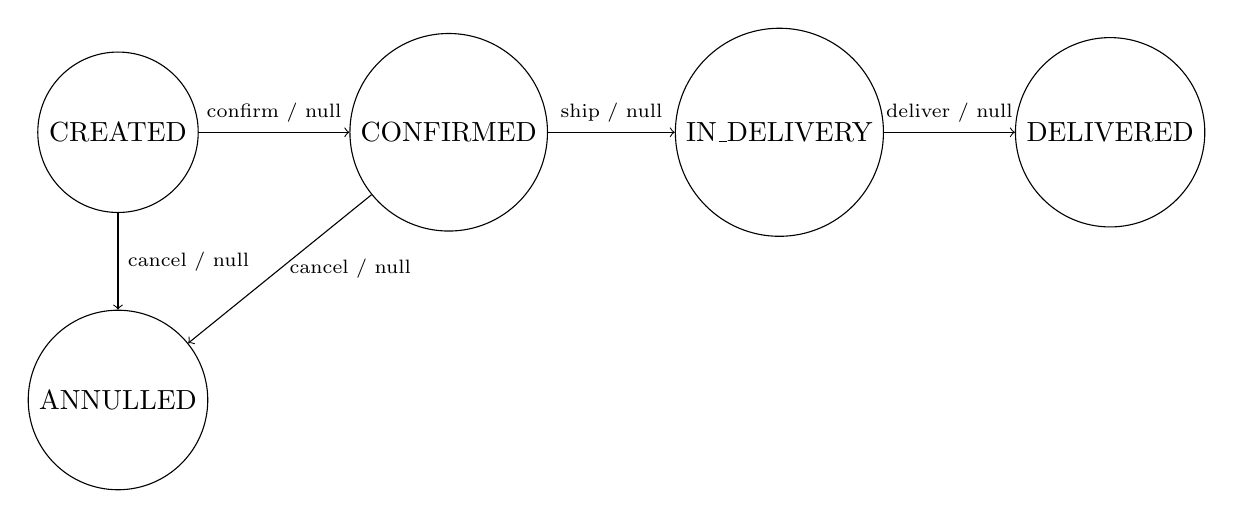
\begin{tikzpicture}[node distance=2cm]
\tikzstyle{st}=[circle,draw,minimum size=1.1cm]
\node[st] (c) {CREATED};
\node[st,right of=c,xshift=2.2cm] (cf) {CONFIRMED};
\node[st,right of=cf,xshift=2.2cm] (in) {IN\_DELIVERY};
\node[st,right of=in,xshift=2.2cm] (del) {DELIVERED};
\node[st,below of=c,yshift=-1.4cm] (an) {ANNULLED};
\draw[->] (c)--(cf) node[midway,above]{\scriptsize confirm / null};
\draw[->] (c)--(an) node[midway,right]{\scriptsize cancel / null};
\draw[->] (cf)--(in) node[midway,above]{\scriptsize ship / null};
\draw[->] (cf)--(an) node[midway,right]{\scriptsize cancel / null};
\draw[->] (in)--(del) node[midway,above]{\scriptsize deliver / null};
\end{tikzpicture}
\caption{State diagram of Ordine (trigger / behaviour, guards mutually
exclusive per BR-04). Implemented via GoF State Pattern in
\texttt{Ordine.cambiaStato()}. Other entities (Ricetta, RuoloVenditore) have
analogous state machines.}
\label{fig:state}
\end{figure}
